\chapter{Accuracy results of the tracking MPC}
\label{app:D}
This appendix shows the results that are discussed in \ref{s:tracking_results}. In red the reference is shown that was derived from \ref{opt:basic_opti_w} with using the bicycle model and in blue the trajectory completed by the Amesim model. During the learning process with the Amesim model (section \ref{s:complex_learning_results}) the first $10 \hspace{1mm}s$ of the Amesim trajectory is thrown away in order to remove the unstable longitudinal behaviour at the start of the simulation.


\begin{figure}[h!]
	\centering
	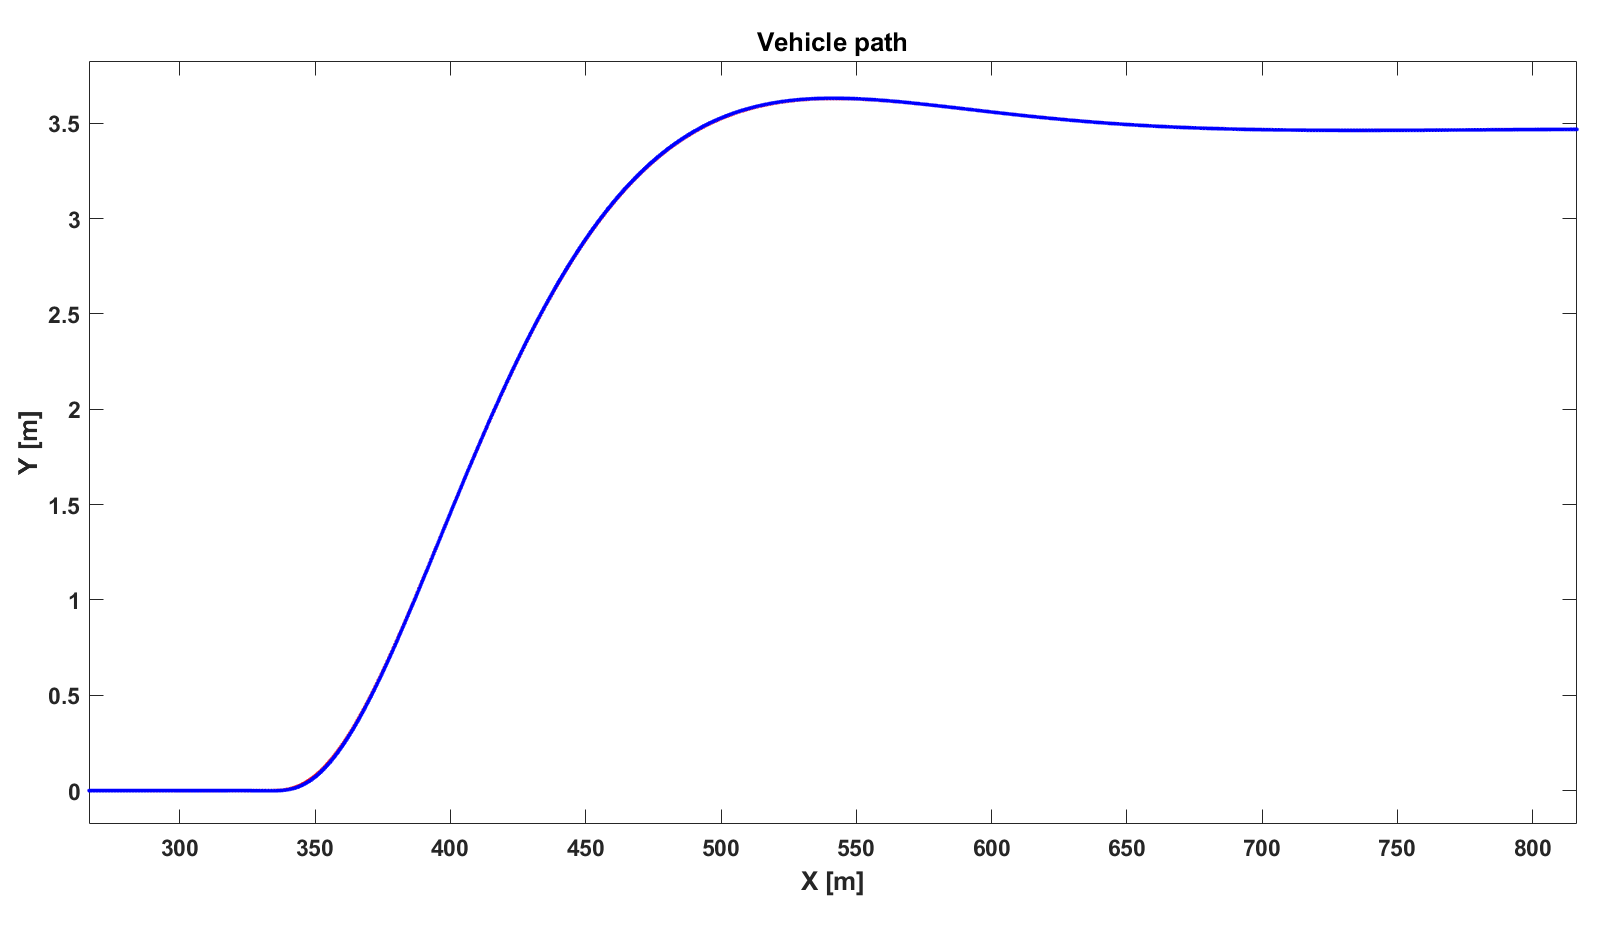
\includegraphics[width=1.15\textwidth]{1path_N50_TMPC C0.1_Tf40.PNG}
\end{figure}

\begin{figure}[h!]
	\centering
	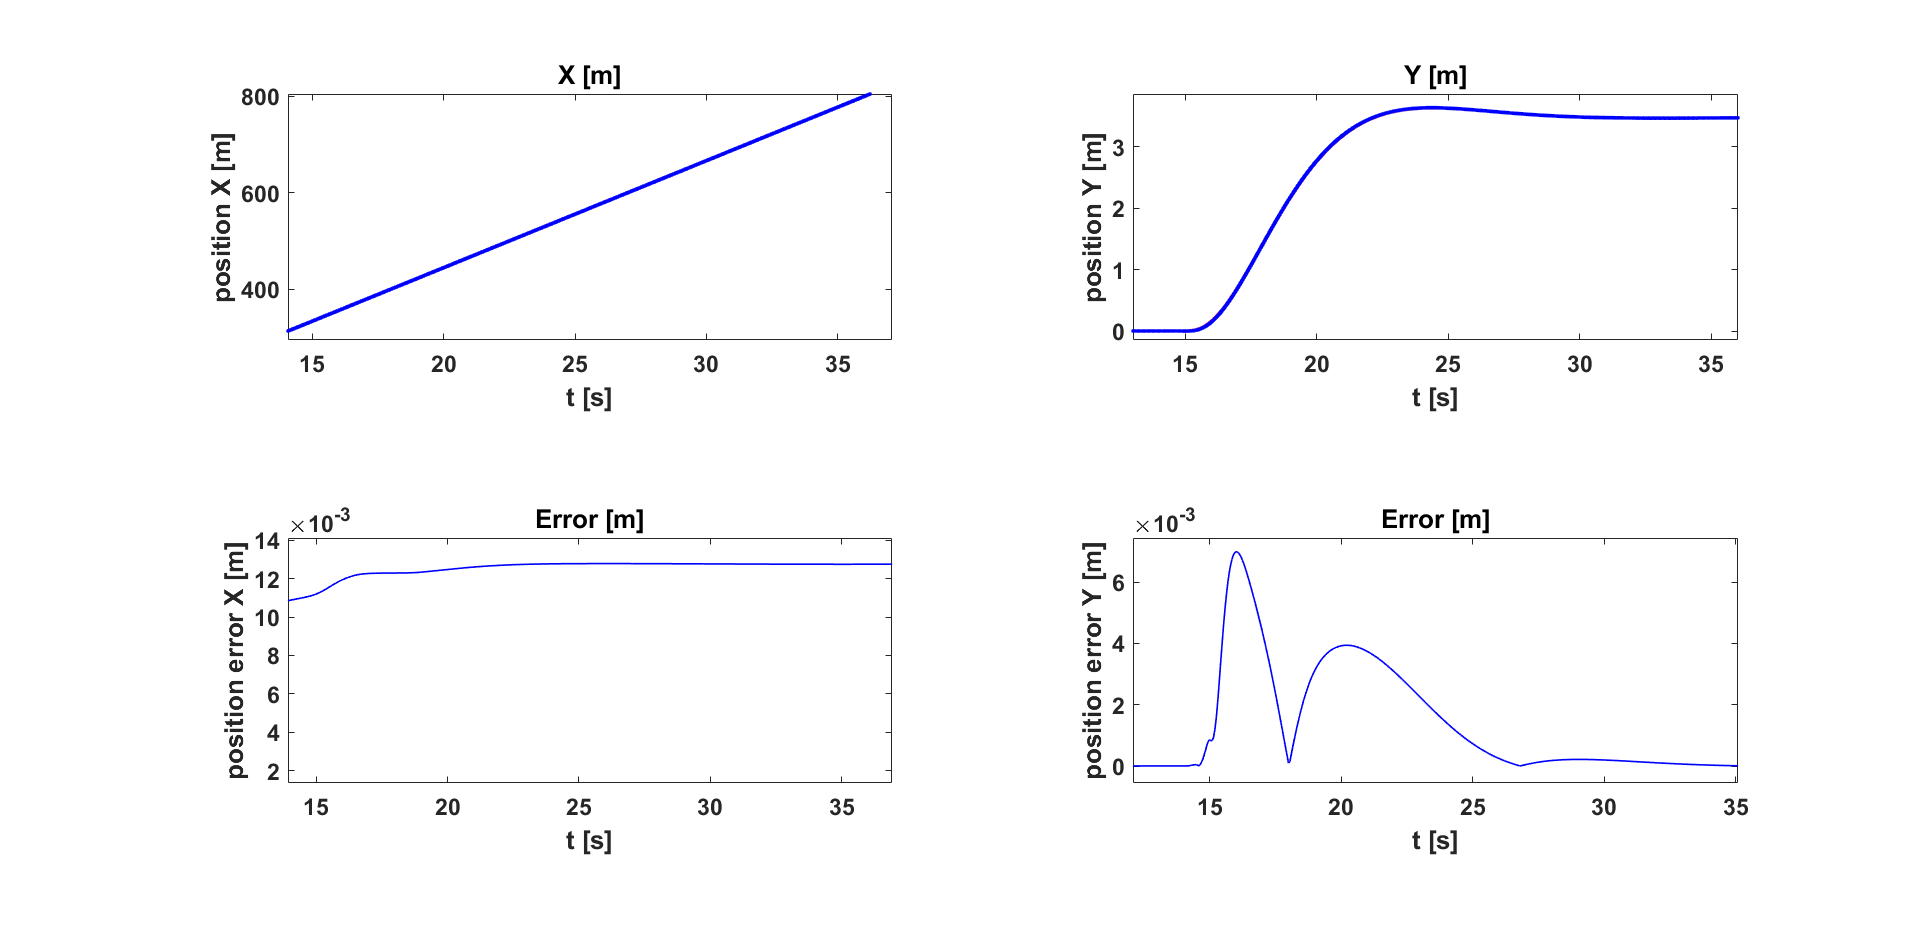
\includegraphics[width=1.15\textwidth]{2xy_N50_TMPC 0.1_Tf40.PNG}
\end{figure}

\begin{figure}[h!]
	\centering
	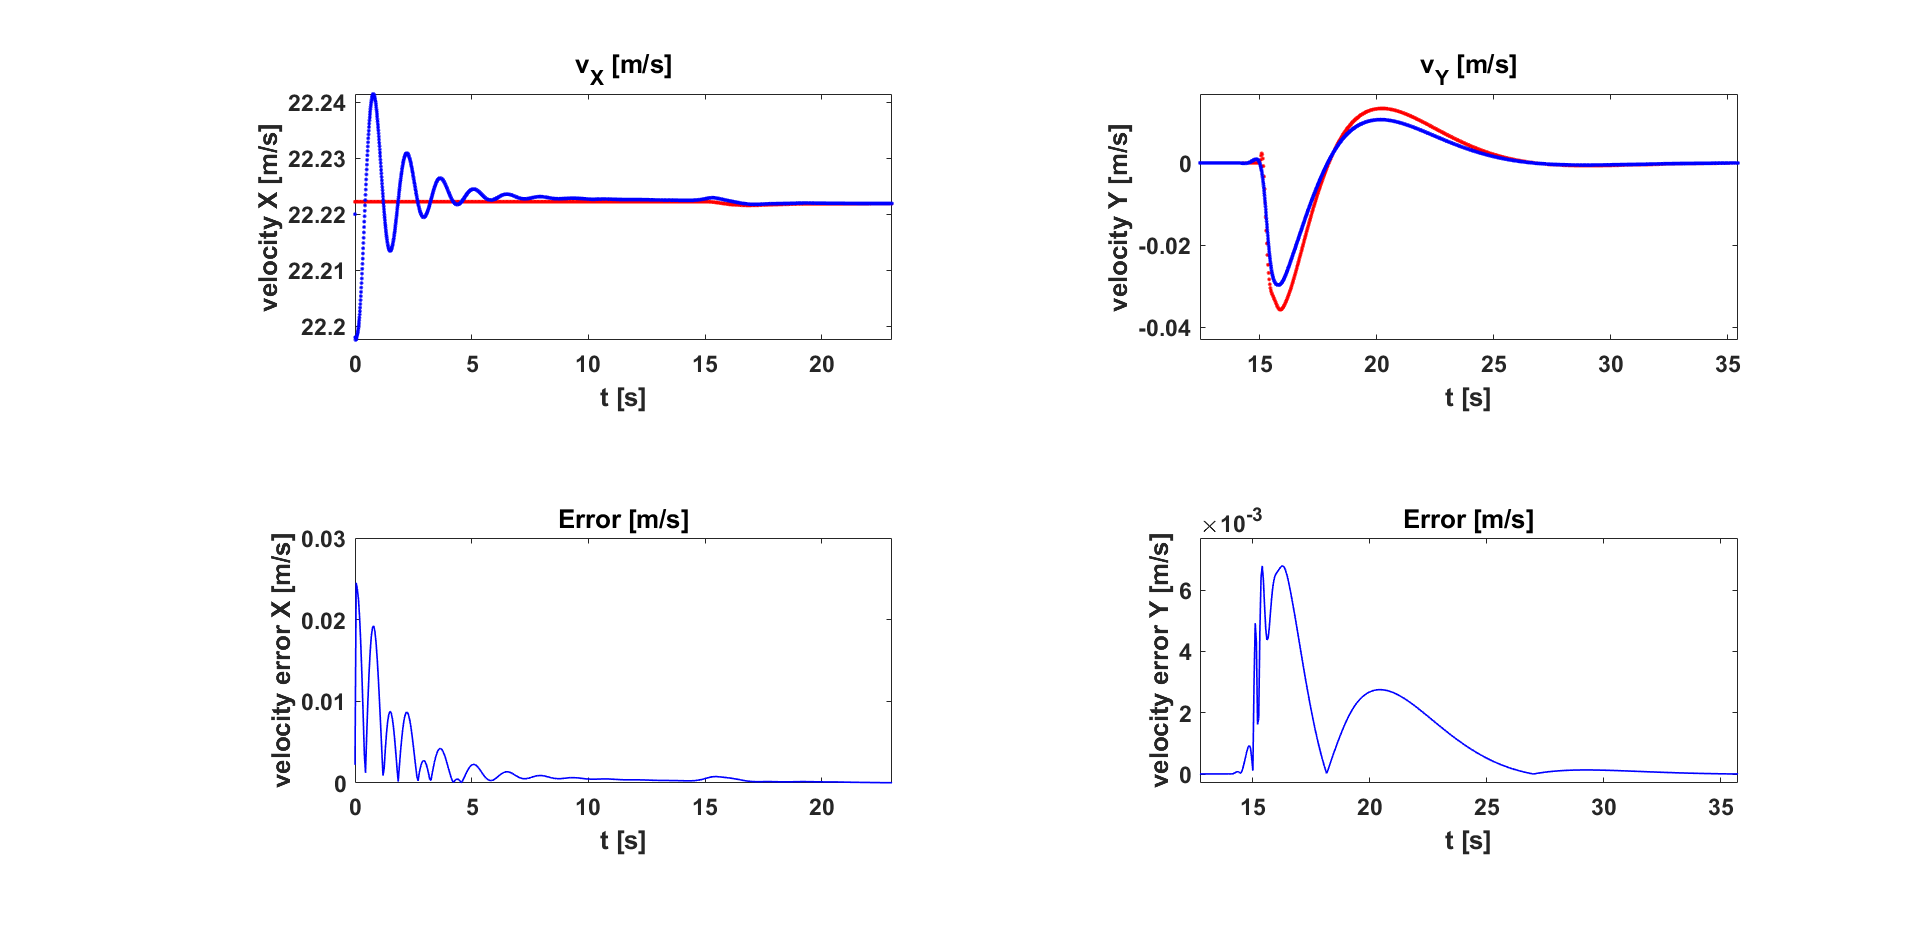
\includegraphics[width=1.15\textwidth]{3vxy_N50_TMPC 0.1_Tf40.PNG}
\end{figure}


\begin{figure}[h!]
	\centering
	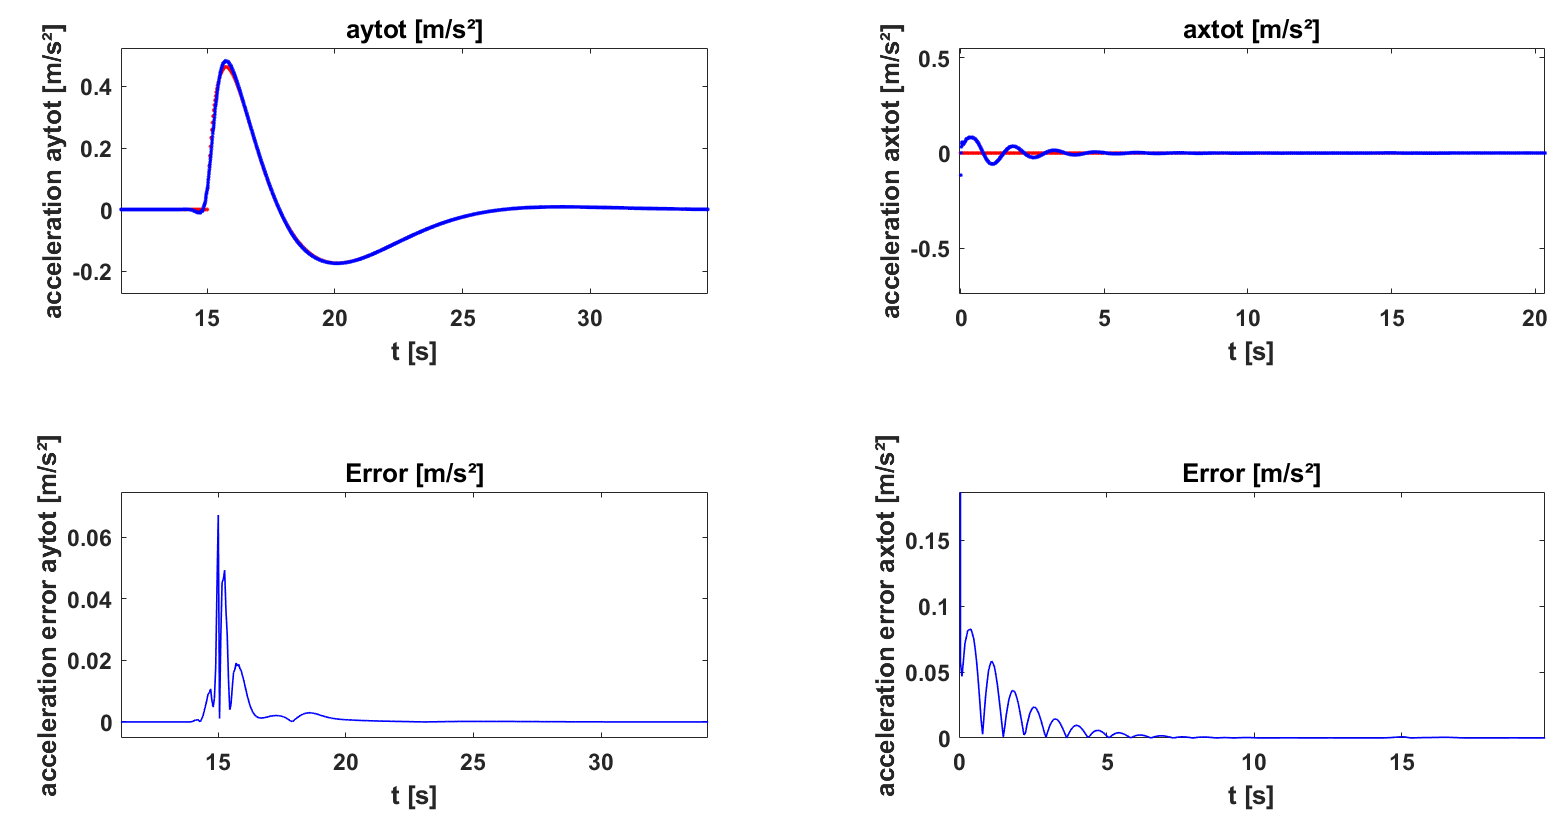
\includegraphics[width=1.15\textwidth]{6atot_N50_TMPC 0.1_Tf40.PNG}
\end{figure}


\begin{figure}[h!]
	\centering
	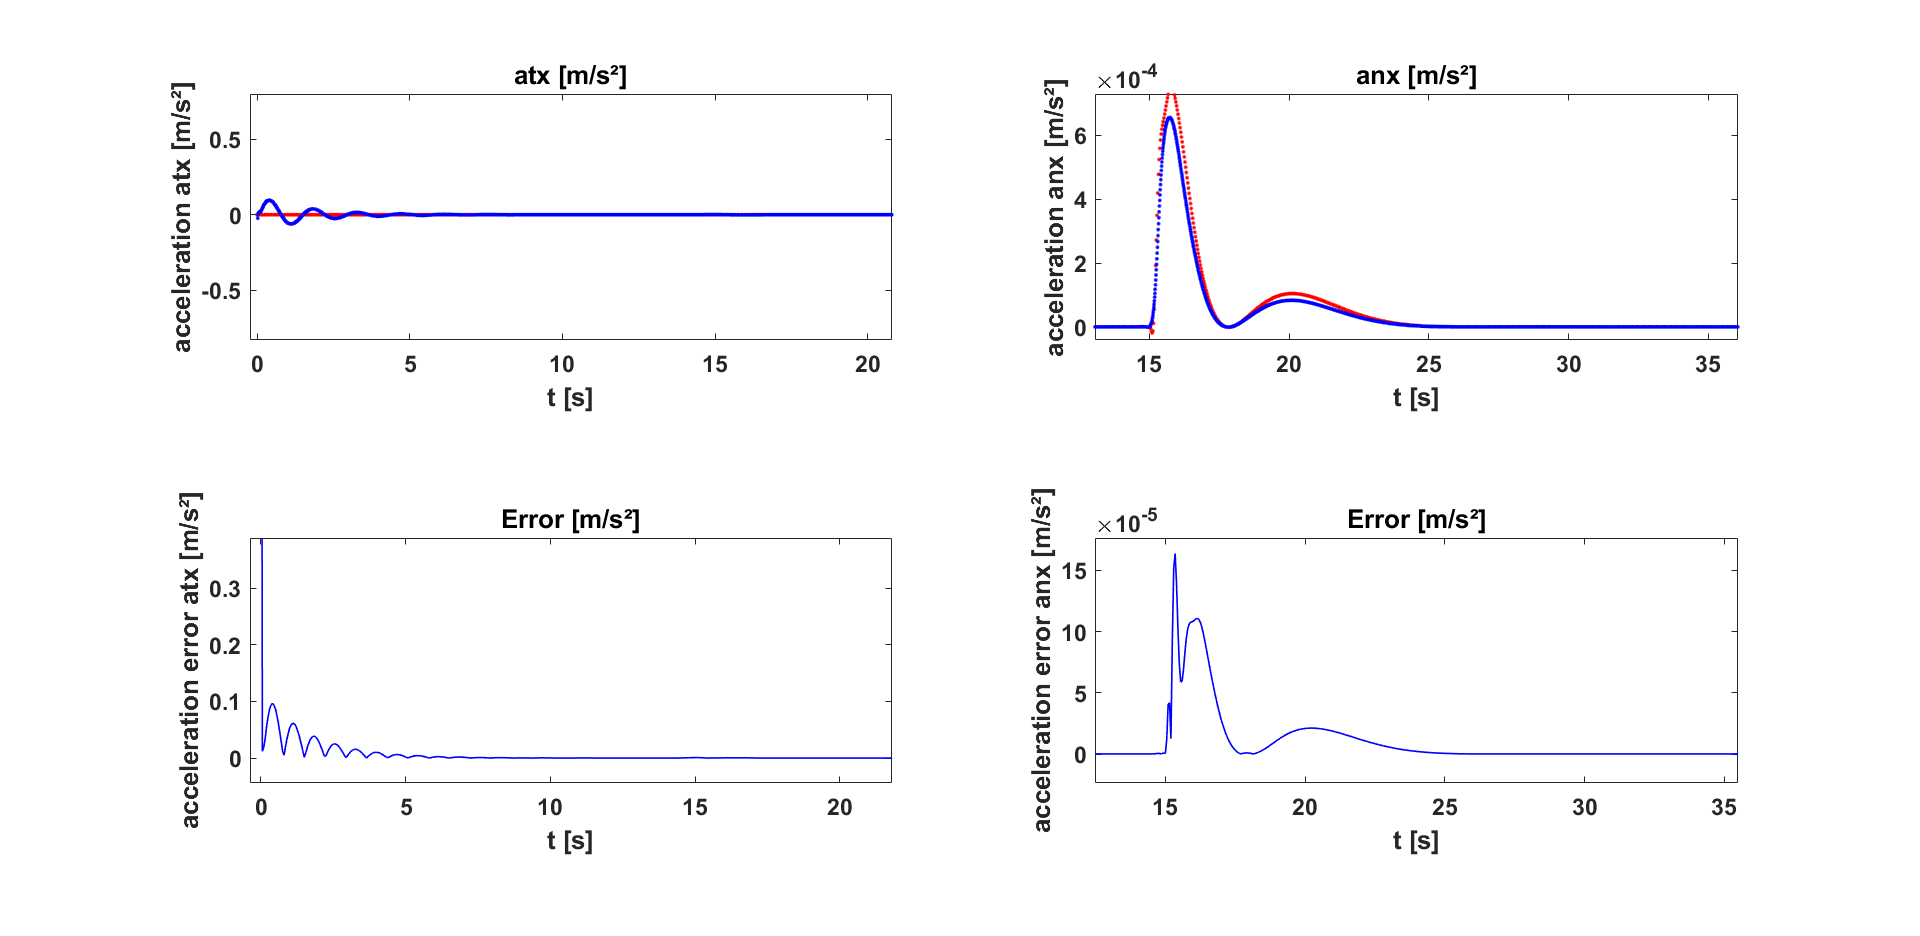
\includegraphics[width=1.15\textwidth]{5ax_N50_TMPC 0.1_Tf40.PNG}
\end{figure}

\begin{figure}[h!]
	\centering
	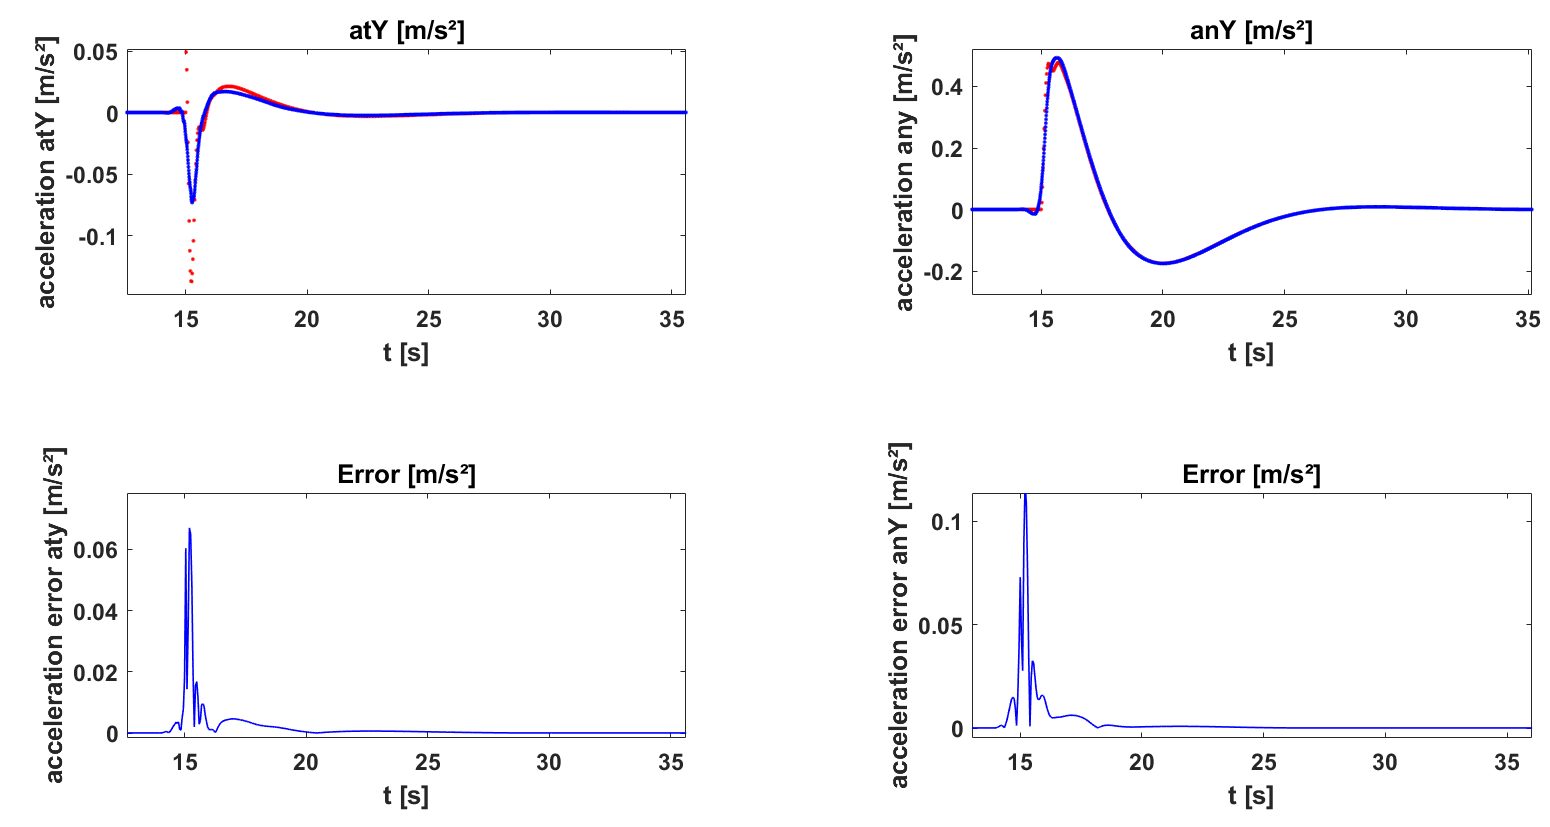
\includegraphics[width=1.15\textwidth]{4ay_N50_TMPC 0.1_Tf40.PNG}
\end{figure}

\begin{figure}[h!]
	\centering
	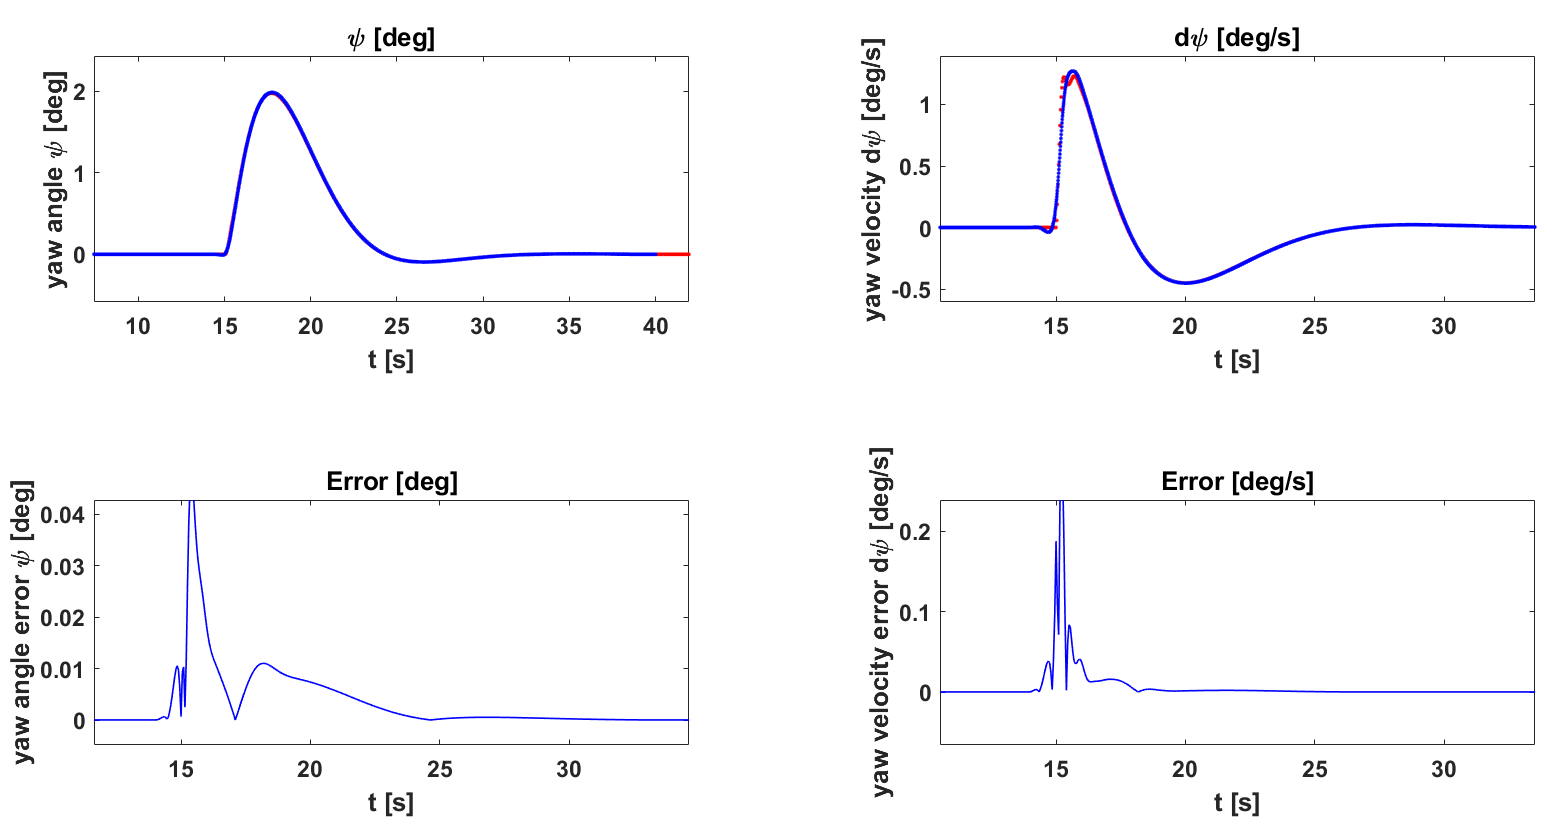
\includegraphics[width=1.15\textwidth]{7psi_N50_TMPC 0.1_Tf40.PNG}
\end{figure}

\begin{figure}[h!]
	\centering
	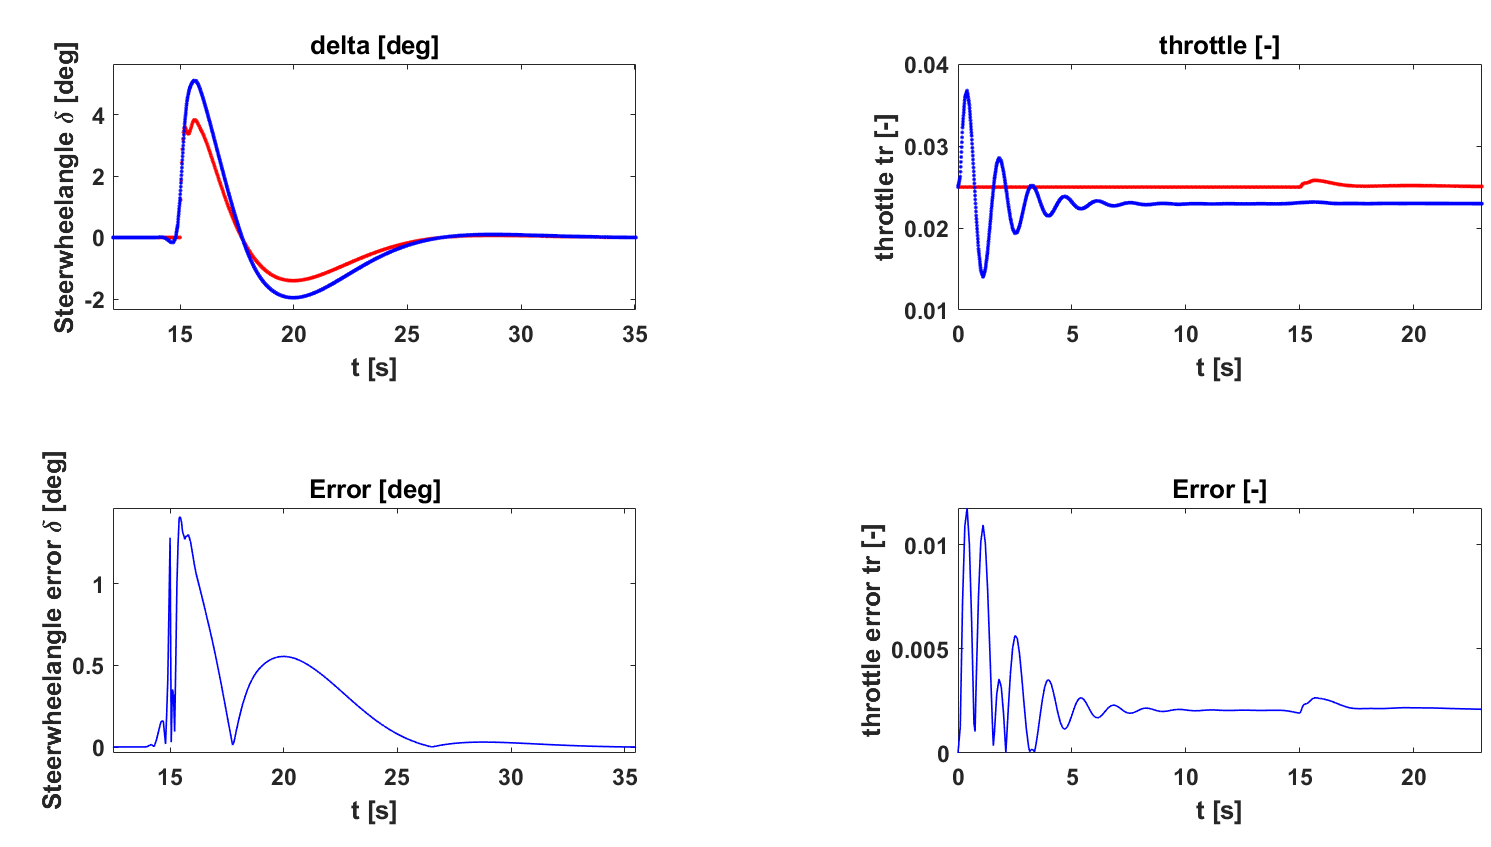
\includegraphics[width=1.15\textwidth]{8tr&delta_N50_TMPC 0.1_Tf40.PNG}
\end{figure}

\begin{figure}[h!]
	\centering
	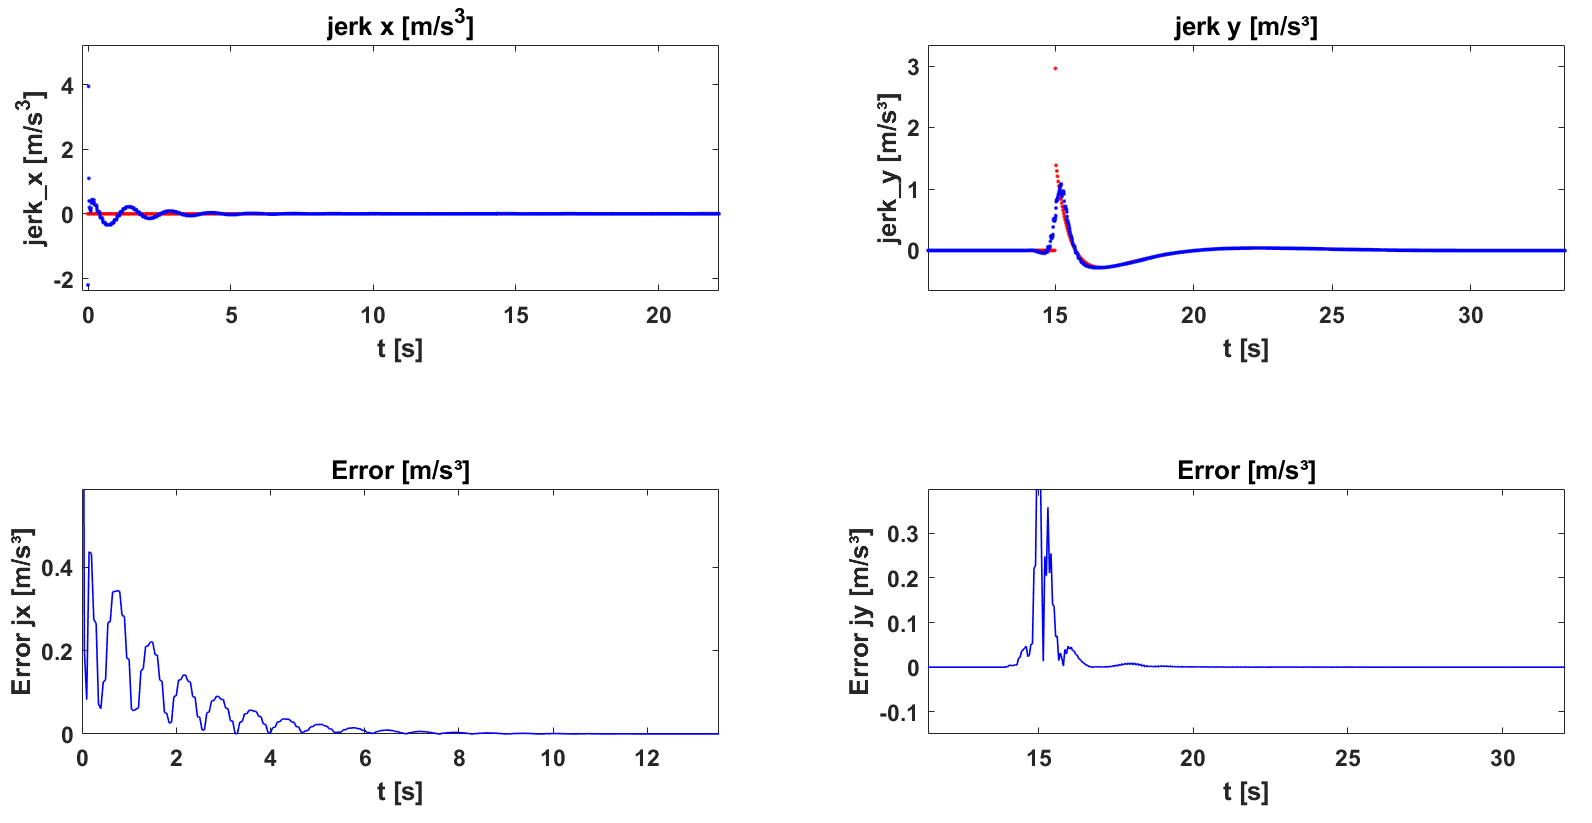
\includegraphics[width=1.15\textwidth]{9jerks_N50_TMPC 0.1_Tf40.PNG}
\end{figure}

\begin{figure}[h!]
	\centering
	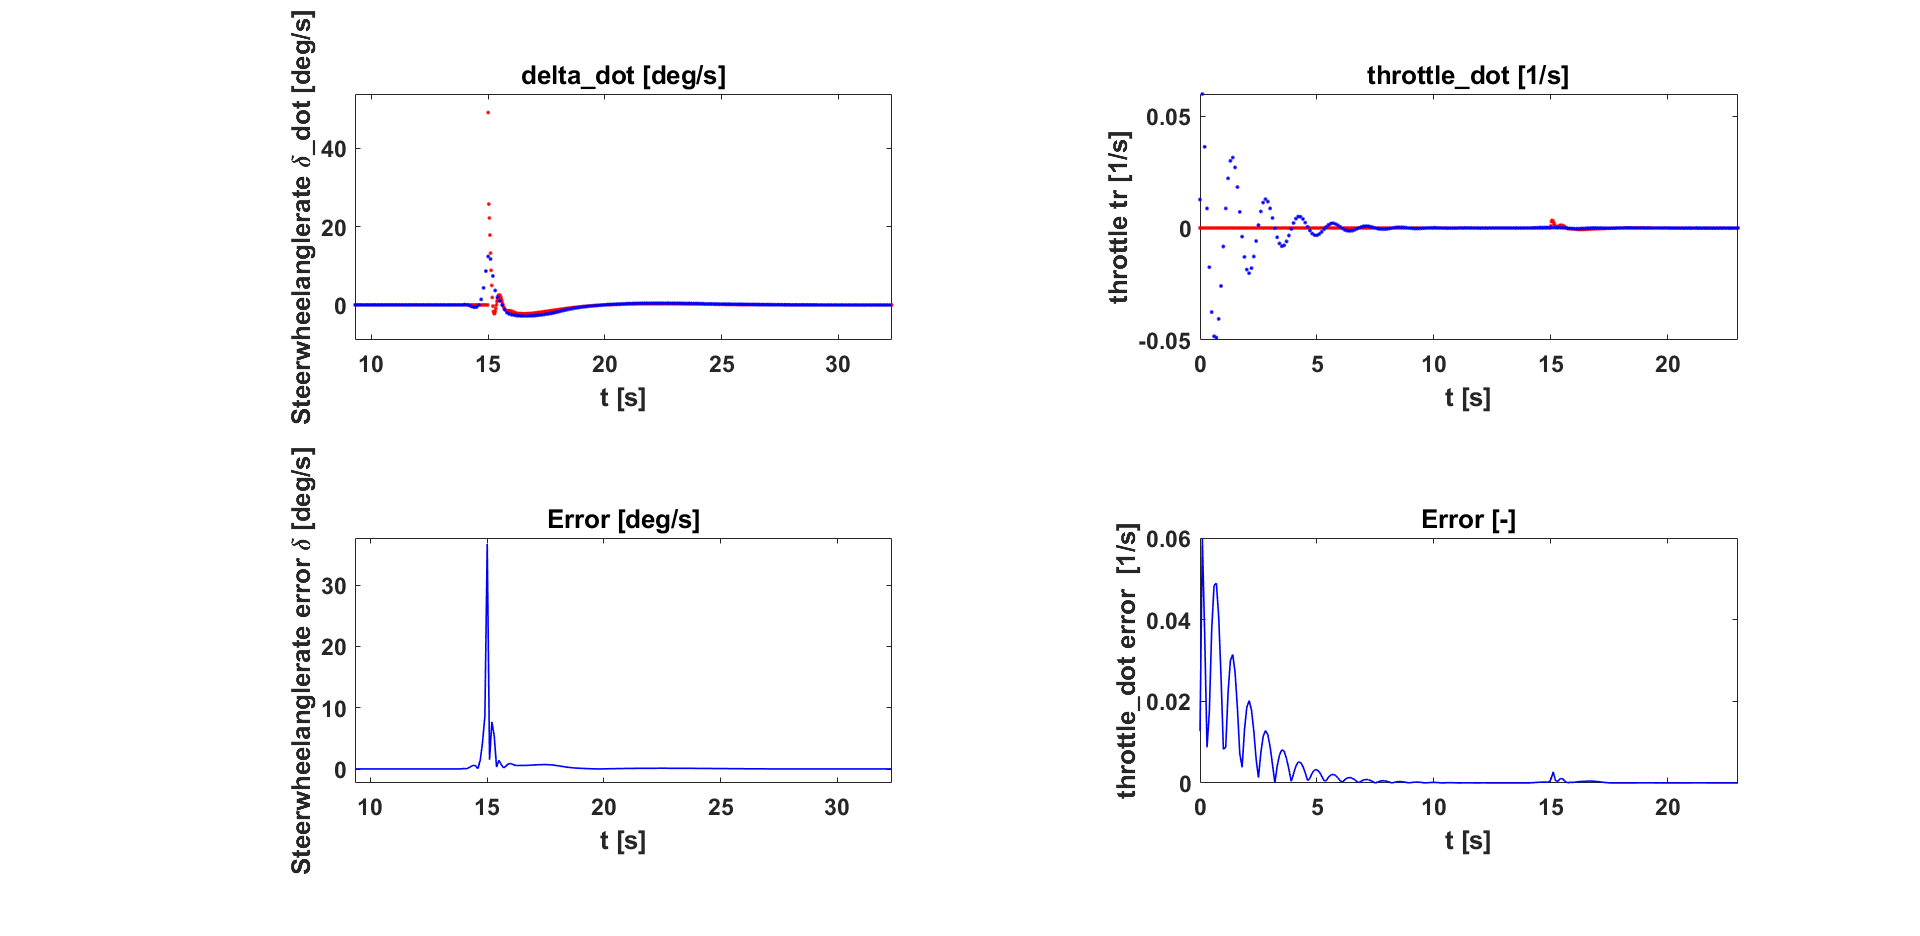
\includegraphics[width=1.15\textwidth]{14tr_dot&delta_dot_N50_TMPC 0.1_Tf40.PNG}
\end{figure}




%%% Local Variables: 
%%% mode: latex
%%% TeX-master: "thesis"
%%% End: 
